%%%%%%%%%%%%%%%%%%%%%%%%%%%%%%%%%%%%%%%%%%%%%%%%%%%%%%%%%%%%%%%%%%%%%%%%%%%

\documentclass[a4paper,oneside,12pt]{article}
\usepackage{mystyle}

\begin{document}

\title{\Large\bf Logarithmic functions}
\author{%%
  Minh Van Nguyen \\
  \url{mvngu@gmx.com}
}
\date{\today}
\maketitle

{\color{red}
\begin{packeditem}
\item Log plot to recognize exponential growth/decay.

\item Newton's law of cooling.

\item Half-life of exponential decay.

\item Use linear regression to estimate parameters of exponential
  model.
\end{packeditem}
}


%%%%%%%%%%%%%%%%%%%%%%%%%%%%%%%%%%%%%%%%%%%%%%%%%%%%%%%%%%%%%%%%%%%%%%%%%%%

\section{What is logarithm?}

You already know that the function $f(x) = 10^x$ is an exponential
function.  Furthermore, the function $f(x)$ represents an exponential
growth.  Suppose you were to solve the equation
%%
\begin{equation}
\label{eqn:exponential_growth_100_10_x}
100
=
10^x.
\end{equation}
%%
Take some time to think about what
\Equation{eqn:exponential_growth_100_10_x} is telling you.  The
equation tells you that you want a value of $x$ such that when $10$ is
raised to the power of $x$, you get $100$ as a result.  What would the
value of $x$ be?  Here, the number $10$ is the \emph{base} and the
unknown $x$ is the \emph{exponent}.  To solve
\Equation{eqn:exponential_growth_100_10_x} for $x$, take the logarithm
to base $10$ of both sides and you get
%%
\begin{equation}
\label{eqn:log10_100}
\log_{10} 100
=
\log_{10} (10^x).
\end{equation}
%%
The right-hand side of \Equation{eqn:log10_100} simplifies to
$\log_{10} (10^x) = x$ because the logarithm is to base $10$ and the
exponential function $10^x$ has base $10$.  In other words,
\Equation{eqn:log10_100} simplifies to
\[
\log_{10} 100
=
x.
\]
If $x = 2$, then $10^2 = 100$.  You say that $2$ is equivalent to the
logarithm of $100$ to base $10$.  In symbol, this is written as
\[
\log_{10}100
=
2.
\]
Thus the solution of \Equation{eqn:exponential_growth_100_10_x} is
$x = 2$.  The discussion is summarised in the next definition.

\begin{definition}
\textbf{Logarithm.}
Let $b$ and $y$ be positive numbers such that $b \neq 1$.  The
\emph{logarithm} to base $b$ of $y$ is equivalent to the exponent $x$
of $b$ such that $b^x = y$.  In symbols, you have $y = b^x$ if
$\log_b y = x$.
\end{definition}

The logarithm to base $10$ of $y > 0$ is written $\log_{10} y$ and is
called the \emph{common logarithm}.  If the base is $2$, then you
write $\log_2 y$, which is also called the \emph{binary logarithm}.
If the base is the irrational number $e$, you write $\log_e y$ and
call this the \emph{natural logarithm}.  Sometimes the natural
logarithm of $y$ is also written as $\ln y$.  Whenever you read about
or use logarithm, make sure that you know what base is used for the
logarithm.  Graphs of the above three logarithmic functions are
illustrated in \Figure{fig:logarithm:graphs}.  Note that
\Equation{eqn:log10_100} uses the common logarithm because the base is
$10$.  The right-hand side of \Equation{eqn:log10_100} simplifies to
$x$ due to \Theorem{thm:logarithm:lob_b_b_power_x} below.

\begin{figure}[!htbp]
\centering
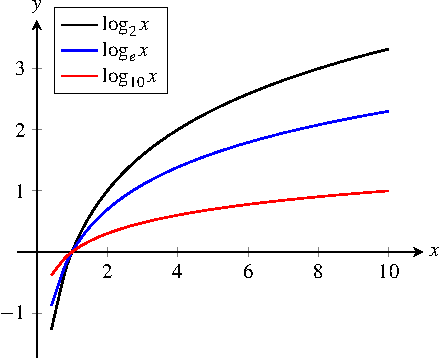
\includegraphics[scale=1.1]{image/12/logarithm.pdf}
\caption{%%
  Graphs of the binary logarithmic function $f(x) = \log_2 x$, the
  natural logarithmic function $f(x) = \log_e x$, and the common
  logarithmic function $f(x) = \log_{10} x$.
}
\label{fig:logarithm:graphs}
\end{figure}

\begin{theorem}
\label{thm:logarithm:lob_b_b_power_x}
Let $b > 0$ be any real number such that $b \neq 1$ and let $x$ be a
real variable.  Then $\log_b (b^x) = x$.
\end{theorem}

Why is \Theorem{thm:logarithm:lob_b_b_power_x} important?
\Theorem{thm:logarithm:lob_b_b_power_x} is often used to solve
equations that involve exponential functions.  In fact, you have
already seen how the theorem was used to solve
\Equation{eqn:exponential_growth_100_10_x} for $x$.  Here are some
more examples.

\begin{example}
Solve the equation $2^x = 64$ for $x$.
\end{example}

\begin{solution}
The equation $2^x = 64$ asks for a value of $x$ such that when $2$ is
raised to the power of $x$, the result will be $64$.  Since the base
is $2$, take the logarithm to base $2$ of both sides of the equation
and you get $\log_2(2^x) = \log_2 64$.  Use
\Theorem{thm:logarithm:lob_b_b_power_x} to simplify the left-hand side
as $\log_2(2^x) = x$, hence you can write $x = \log_2 64$.  You can
use a calculator or computer program to determine that
$x = \log_2 64 = 6$.  As a check, you can see that $2^6 = 64$.
\end{solution}

\begin{example}
\textbf{Population of Australia.}
According to the Australian Bureau of Statistics~(ABS), at the end of
September 2017 the population of Australia grew by $1.6\%$ since the
previous year.\footnote{
  ``3101.0 - Australian Demographic Statistics, Sep 2017'',
  \url{http://web.archive.org/web/20180420062713/http://www.abs.gov.au/AUSSTATS/abs@.nsf/Lookup/3101.0Main+Features1Sep\%202017},
  accessed 2018-04-20.
}
The population by the end of the given period was estimated to be
$24.7029$ million people.  Assume that for the next few years the
population of Australia will grow by a constant rate of $1.6\%$ per
annum.  When will the population of Australia be $30$ million people?
\end{example}

\begin{solution}
You have seen this example before and know that the population~(in
millions) in $t$ years from $2017$ onwards can be written as
\[
P(t)
=
24.7029 \times 1.016^t.
\]
Note that the base is $b = 1.016$.  You want to determine the number
of years $t$ such that $P(t) = 30$ million people.  In other words,
you want to solve the equation
\[
30
=
24.7029 \times 1.016^t
\]
for $t$.  Divide both sides by $24.7029$ to get
$\frac{30}{24.7029} = 1.016^t$.  Now take the logarithm to base
$b = 1.016$ of both sides and you end up with
\[
\log_{1.016} \frac{30}{24.7029}
=
\log_{1.016} (1.016^t).
\]
Use \Theorem{thm:logarithm:lob_b_b_power_x} to simplify the right-hand
side to $\log_{1.016} (1.016^t) = t$ and you can now write
%%
\begin{equation}
\label{eqn:logarithm:Australia_population_doubling_time}
\log_{1.016} \frac{30}{24.7029}
=
t.
\end{equation}
%%
The latter expression evaluates to approximately $t \approx 12.2392$,
rounded to four decimal places.  As a check, you can see that in
approximately $t = 12.2392$ years the population of Australia will be
\[
24.7029 \times 1.016^{12.2392}
\approx
30.000011
\]
million people, rounded to six decimal places.  Therefore some time in
the year $2017 + 12 = 2029$ the population of Australia will be
approximately $30$ million people.
\end{solution}

\begin{exercise}
\textbf{Bacterial growth.}
A Petri dish initially contains ten cells of a type of bacteria.  The
bacteria population is known to have a constant percentage growth rate
of $56\%$ per hour.
%%
\begin{packedenum}
\item\label{subex:logarithm:bacterial_growth_at_least_100_cells}
  Use logarithm to calculate the amount of time required for the
  bacteria population to be at least $100$ cells.

\item\label{subex:logarithm:bacterial_growth_doubling_time}
  Use logarithm to calculate the doubling time of the bacteria
  population.
\end{packedenum}
\end{exercise}

\ifbool{showSolution}{
\begin{solution}
\solutionpart{subex:logarithm:bacterial_growth_at_least_100_cells}
From a previous example, you know that the bacteria population can be
written as $Q(t) = 10 \times 1.56^t$.  Now you want to solve the
equation
\[
100
=
10 \times 1.56^t
\]
for $t$.  Divide both sides of the latter equation by $10$ to get
$\frac{100}{10} = 1.56^t$, which simplifies to $10 = 1.56^t$.  In the
exponential function $1.56^t$, the base is $b = 1.56$.  Take the
logarithm to base $b = 1.56$ of both sides of $10 = 1.56^t$ and you
end up with $\log_{1.56} 10 = \log_{1.56} (1.56^t)$, which by
\Theorem{thm:logarithm:lob_b_b_power_x} can be simplified as
$\log_{1.56} 10 = t$.  Thus $t$ is approximately $t \approx 5.1780$,
rounded to four decimal places.  As a check, note that
$Q(5.1780) = 10 \times 1.56^{5.1780} \approx 99.9998$, rounded to four
decimal places.  However, if $t = 5.1781$ then you have
$Q(5.1781) = 10 \times 1.56^{5.1781} \approx 100.0043$, rounded to
four decimal places.  In other words, you must wait a minimum of
$5.1781$ hours in order for the bacteria population to be at least
$100$ cells.

\solutionpart{subex:logarithm:bacterial_growth_doubling_time}
The initial bacteria population is $a = 10$ cells.  Double this and
you get $2a = 2 \times 10 = 20$ cells.  You want to know the amount of
time required in order for the bacteria population to double from $10$
cells to $20$ cells.  That is, you want to solve the equation
\[
20
=
10 \times 1.56^t
\]
for $t$.  Divide both sides of the latter equation by $10$ to get
$\frac{20}{10} = 1.56^t$, which simplifies to $2 = 1.56^t$.  Taking
the logarithm to base $b = 1.56$ of both sides yields
$\log_{1.56} 2 = \log_{1.56} (1.56^t)$ and use
\Theorem{thm:logarithm:lob_b_b_power_x} to simplify the last equation
to $\log_{1.56} 2 = t$.  Then $t$ is approximately
$t \approx 1.5587$, rounded to four decimal places.  As a check, you
have $Q(1.5587) = 10 \times 1.56^{1.5587} \approx 19.9997$, rounded to
four decimal places.  However, if $t = 1.5588$ then you get
$Q(1.5588) = 10 \times 1.56^{1.5588} \approx 20.0006$, rounded to four
decimal places.  Conclude that the doubling time of the bacteria
population is approximately $1.5588$ hours.
\end{solution}
}{}

\begin{example}
\textbf{Radiocarbon dating.}
Carbon-$14$ decays at a rate of approximately $r = 0.00012097$ per
annum, rounded to eight decimal places.  Calculate the half-life of
$300$ isotopes of carbon-$14$.
\end{example}

\begin{solution}
Radioactive decay follows an exponential decay model of the form
\[
A(t)
=
a e^{-rt}.
\]
Here, $a$ represents the initial number of radioactive isotopes, $r$
denotes the decay rate as a decimal, and $A(t)$ represents the
remaining number of radioactive isotopes after $t$ units of time.  In
the example, you initially have $a = 300$ isotopes of carbon-$14$ and
the decay rate is $r = 0.00012097$ per annum.  After $t$ years, the
number of remaining carbon-$14$ isotopes can be written as
\[
A(t)
=
300 e^{-0.00012097 t}.
\]
You want to know the number of years required for the initial $300$
isotopes to decay to $\frac{300}{2} = 150$ isotopes.  That is, you
want to solve the equation
\[
150
=
300 e^{-0.00012097 t}
\]
for $t$.  Divide both sides by $300$ to get
$\frac{150}{300} = e^{-0.00012097 t}$, which simplifies to
$\frac{1}{2} = e^{-0.00012097 t}$.  In the exponential function
$e^{-0.00012097 t}$, the base is the irrational number $e$.  Take the
logarithm to base $e$ of both sides of
$\frac{1}{2} = e^{-0.00012097 t}$ and you end up with
$\ln \bigparen{\frac{1}{2}} = \ln \bigparen{e^{-0.00012097 t}}$,
which by \Theorem{thm:logarithm:lob_b_b_power_x} simplifies to
$\ln \bigparen{\frac{1}{2}} = -0.00012097 t$.  Solving the latter
equation for $t$ yields
\[
-\frac{1}{0.00012097}
\ln \parenthesis*{\frac{1}{2}}
=
t
\]
which evaluates to approximately $t \approx 5730$ years, rounded to
the nearest integer.  Conclude that the initial $300$ carbon-$14$
isotopes have a half-life of approximately $5730$ years.
\end{solution}

\begin{exercise}
\textbf{Fermium-$250$.}
Fermium-$250$ is known to have a decay rate of approximately $0.0231$
per minute.  Calculate the half-life of $100$ isotopes of
fermium-$250$.
\end{exercise}

\ifbool{showSolution}{
\begin{solution}
If $A(t)$ represents the number of remaining fermium-$250$ isotopes
after $t$ minutes, then $A(t)$ can be written as
\[
A(t)
=
100 e^{-0.0231 t}.
\]
Half of $100$ is $100 / 2 = 50$ and you want to solve the equation
\[
50
=
100 e^{-0.0231 t}
\]
for $t$.  In the latter equation, divide both sides by $100$ to get
$\frac{50}{100} = e^{-0.0231 t}$, which simplifies to
$\frac{1}{2} = e^{-0.0231 t}$.  Take the logarithm to base $e$ of both
sides and you end up with
$\ln \parenthesis*{\frac{1}{2}} = \ln \parenthesis*{e^{-0.0231 t}}$,
which by \Theorem{thm:logarithm:lob_b_b_power_x} simplifies to
$\ln \parenthesis*{\frac{1}{2}} = -0.0231 t$.  The last equation
can be solved for $t$ to get
\[
t
=
-\frac{1}{0.0231}
\ln \parenthesis*{\frac{1}{2}}
\]
which evaluates to approximately $t \approx 30$, rounded to the
nearest integer.  Therefore the half-life of $100$ isotopes of
fermium-$250$ is approximately $30$ minutes.
\end{solution}
}{}


%%%%%%%%%%%%%%%%%%%%%%%%%%%%%%%%%%%%%%%%%%%%%%%%%%%%%%%%%%%%%%%%%%%%%%%%%%%

\section{Properties of logarithm}

One of the most useful properties of logarithm is that exponentiation
and logarithm are inverse functions of each other.  This is similar to
the way addition and subtraction are inverse operations of each other,
or multiplication and division are inverse operations of each other.
Consequently, you can use this inverse property between exponentiation
and logarithm to solve equations that involve exponential and
logarithmic functions.  What does all this mean?

Consider the example of addition and subtraction.  Suppose you have
two numbers $a$ and $x$ such that $a \neq 0$.  Adding $a$ to $x$
results in $x + a$.  You can undo the addition by subtracting $a$ from
$x + a$.  Doing so gives you the expression
\[
(x + a) - a
=
x + a - a
=
x.
\]
On the other hand, suppose you subtract $a$ from $x$ and end up with
$x - a$.  Undoing the subtraction requires that you add $a$ to
$x - a$.  Doing so results in
\[
(x - a) + a
=
x - a + a
=
x.
\]
The core idea is that addition and subtraction are inverse operations
of each other.  This inverse property between addition and subtraction
allows you to undo the result of any of the two operations.

As another example, consider multiplication and division.  Let $a$ and
$x$ be any numbers such that $a \neq 0$ and $x \neq 0$.  Multiplying
$x$ by $a$ results in $ax$.  To undo the multiplication, you divide
$ax$ by $a$ to produce
\[
\frac{ax}{a}
=
\frac{a}{a} \times x
=
x.
\]
On the other hand, suppose that you divide $x$ by $a$ to get $x / a$.
To undo the division, you multiply $x / a$ by $a$ to get
\[
\frac{x}{a} \times a
=
\frac{a}{a} \times x
=
x.
\]
Thus you see that multiplication and division are inverse operations
of each other.  This inverse property between multiplication and
division allows you to undo the result of any of the two operations.

The fact that exponentiation and logarithm are inverses of each other
is summarised in \Theorem{thm:logarithm:lob_b_b_power_x}.  This
inverse property between exponentiation and logarithm can be
visualised as the graph shown in
\Figure{fig:logarithmic_function_reflection_of_exponential_function}
for the specific case of the natural logarithmic function
$f(x) = \ln x$ and the exponential function $g(x) = e^x$.  The graphs
for exponentiation and logarithm to other bases are similar.
\Figure{fig:logarithmic_function_reflection_of_exponential_function}
shows that you can obtain the graph of $g(x)$ by reflecting the graph
of $f(x)$ about the diagonal line $y = x$.  Furthermore, you can also
produce the graph of $f(x)$ by reflecting the graph of $g(x)$ about
the line $y = x$.  This means that, for example, given the point
$\tuple{0}{1}$ on the graph of $g(x)$, the corresponding point on the
graph of $f(x)$ is obtained by interchanging the $x$- and
$y$-coordinates to get $\tuple{1}{0}$.  In fact,
\Theorem{thm:logarithm:lob_b_b_power_x} is part of another theorem
that can be used to cancel exponentiation and logarithm whenever these
two operations occur together.  This other result is
\Theorem{thm:logarithm:cancellation_property} below.

\begin{figure}[!htbp]
\centering
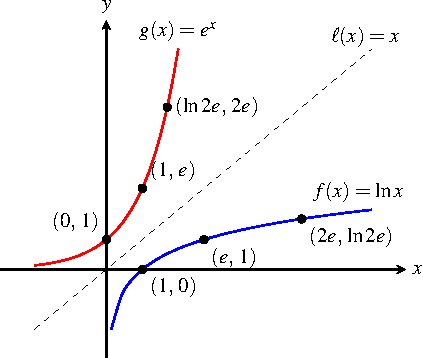
\includegraphics[scale=1.2]{image/12/inverses.pdf}
\caption{%%
  The graph of the natural logarithmic function $f(x) = \ln x$ is
  obtained by reflecting the exponential function $g(x) = e^x$ with
  respect to the line $\ell(x) = x$.
}
\label{fig:logarithmic_function_reflection_of_exponential_function}
\end{figure}

\begin{exercise}
Provide an example of two operations~(different from those presented
above) that are inverses of each other.  Explain how one operation can
be used to undo the result of the other operation.
\end{exercise}

\ifbool{showSolution}{
\begin{solution}
The operations of squaring and square root are inverses of each
other.  Let $x \geq 0$ be any real number.  The square of $x$ is
$x^2$.  To undo the squaring, take the square root of $x^2$ and you
get
\[
\sqrt{x^2}
=
(x^2)^{1/2}
=
x^{2/2}
=
x.
\]
On the other hand, the square root of $x$ is $\sqrt{x}$.  To undo the
square root, you square $\sqrt{x}$ and end up with
\[
\bigparen{\sqrt{x}}^2
=
\bigparen{x^{1/2}}^2
=
x^{2/2}
=
x.
\]
Thus either operation can be used to undo the result of the other
operation.
\end{solution}
}{}

\begin{theorem}
\label{thm:logarithm:cancellation_property}
\textbf{Cancellation property.}
Let $b$ be a positive number such that $b \neq 1$.
%%
\begin{packedenum}
\item\label{subthm:logarithm:cancellation_property_log_exponential}
  If $x$ is any real number, then $\log_b (b^x) = x$.

\item\label{subthm:logarithm:cancellation_property_exponential_log}
  If $x > 0$ is any positive number, then $b^{\log_b x} = x$.
\end{packedenum}
\end{theorem}

\begin{example}
Solve the equation $\log_{10} x = \frac{1}{2}$ for $x$.
\end{example}

\begin{solution}
The equation $\log_{10} x = \frac{1}{2}$ asks you to determine a value
of $x$ such that $\log_{10} x$ evaluates to $1 / 2$.  You can use
\Subtheorem{thm:logarithm:cancellation_property}{subthm:logarithm:cancellation_property_exponential_log}
and consider both sides of $\log_{10} x = \frac{1}{2}$ as exponents of
the base $10$.  Then the latter equation can be written as
\[
10^{\log_{10} x}
=
10^{1/2}
=
\sqrt{10}.
\]
The left-hand side simplifies to $x$ and the equation now becomes
$x = \sqrt{10}$.
\end{solution}

\begin{exercise}
Solve the equation $\log_2 x = 5$ for $x$.
\end{exercise}

\ifbool{showSolution}{
\begin{solution}
You can treat both sides of $\log_2 x = 5$ as exponents of the base
$2$.  Then the latter equation can also be written as
\[
2^{\log_2 x}
=
2^5
\]
which by
\Subtheorem{thm:logarithm:cancellation_property}{subthm:logarithm:cancellation_property_exponential_log}
simplifies to $x = 2^5 = 32$.
\end{solution}
}{}

\begin{exercise}
Solve the equation $\ln 2x = 3$ for $x$.
\end{exercise}

\ifbool{showSolution}{
\begin{solution}
You can treat both sides of the equation $\ln 2x = 3$ as exponents of
the irrational number $e$.  This allows you to write the latter
equation as
\[
e^{\ln 2x}
=
e^3.
\]
Use
\Subtheorem{thm:logarithm:cancellation_property}{subthm:logarithm:cancellation_property_exponential_log}
to simplify the last equation to $2x = e^3$, which upon solving for
$x$ yields $x = \frac{1}{2} e^3$.
\end{solution}
}{}

\begin{theorem}
\label{thm:logarithm:properties}
\textbf{Properties of logarithm.}
Let $\triple{a}{b}{c}$ be positive numbers such that $b \neq 1$.
%%
\begin{packedenum}
\item\label{thm:logarithm:properties_addition}
  Addition rule:
  $\log_b (ac) = \log_b a + \log_b c$

\item\label{thm:logarithm:properties_subtraction}
  Subtraction rule:
  $\log_b \parenthesis*{\frac{a}{c}} = \log_b a - \log_b c$

\item\label{thm:logarithm:properties_multiplication}
  Power rule:
  If $x$ is any real number, then $\log_b (a^x) = x \cdot \log_b a$.

\item\label{thm:logarithm:properties_log_1}
  Zero rule: $\log_b 1 = 0$

\item\label{thm:logarithm:properties_log_b}
  Unit rule: $\log_b b = 1$
\end{packedenum}
\end{theorem}

\begin{proof}
\solutionpart{thm:logarithm:properties_addition}
Since $\triple{a}{b}{c}$ are positive numbers, there exist numbers $m$
and $n$ such that $a = b^m$ and $c = b^n$.  By
\Subtheorem{thm:logarithm:cancellation_property}{subthm:logarithm:cancellation_property_log_exponential}
you have the identities
%%
\begin{equation}
\label{eqn:logarithm:log_b_a_m_log_b_c_n}
\log_b a = \log_b (b^m) = m
%%
\qquad
\text{and}
\qquad
%%
\log_b c = \log_b (b^n) = n.
\end{equation}
%%
The product of $a$ and $c$ can be written as
$a \cdot c = b^m \cdot b^n$, which simplifies to
$a \cdot c = b^{m + n}$.  In the latter equation, taking the logarithm
to base $b$ of both sides results in
$\log_b (a \cdot c) = \log_b (b^{m+n})$.  Use
\Subtheorem{thm:logarithm:cancellation_property}{subthm:logarithm:cancellation_property_log_exponential}
again to simplify the last equation to $\log_b (a \cdot c) = m+n$,
which by the identities in~\eqref{eqn:logarithm:log_b_a_m_log_b_c_n}
can be written as
$\log_b (a \cdot c) = \log_b a + \log_b c$.

\solutionpart{thm:logarithm:properties_subtraction}
See \Exercise{ex:logarithm:properties_subtraction}.

\solutionpart{thm:logarithm:properties_multiplication}
Since $a$ and $b$ are positive numbers, there exists a number $n$ such
that $a = b^n$.  If $x$ is any real number, raise both sides of the
latter equation to the power of $x$ and you get
$a^x = (b^n)^x$, which simplifies to $a^x = b^{nx}$.  In the last
equation, take the logarithm to base $b$ of both sides and you obtain
$\log_b (a^x) = \log_b (b^{nx})$, which by
\Subtheorem{thm:logarithm:cancellation_property}{subthm:logarithm:cancellation_property_log_exponential}
can also be written as
%%
\begin{equation}
\label{eqn:logarithm:log_b_a_x_nx}
\log_b (a^x)
=
nx.
\end{equation}
%%
In the equation $a = b^n$, taking the logarithm to base $b$ of both
sides produces $\log_b a = \log_b (b^n)$ and using
\Subtheorem{thm:logarithm:cancellation_property}{subthm:logarithm:cancellation_property_log_exponential}
again shows that you can also write $\log_b a = n$.  Substitute the
latter expression into \Equation{eqn:logarithm:log_b_a_x_nx} and you
get $\log_b (a^x) = (\log_b a) \cdot x$, which you can also write as
$\log_b (a^x) = x \cdot \log_b a$.

\solutionpart{thm:logarithm:properties_log_1}
See \Exercise{ex:logarithm:log_b_1_0}.

\solutionpart{thm:logarithm:properties_log_b}
As $b \neq 1$ is positive, use
\Subtheorem{thm:logarithm:cancellation_property}{subthm:logarithm:cancellation_property_exponential_log}
to write $b^{\log_b b} = b$.  Taking the logarithm to base $b$ of both
sides yields $\log_b (b^{\log_b b}) = \log_b b$, which by the power
rule from \Part{thm:logarithm:properties_multiplication} can also be
written as $\log_b b \cdot \log_b b = \log_b b$.  Since $b \neq 1$,
by \Part{thm:logarithm:properties_log_1} you know that
$\log_b b \neq 0$.  Thus in the equation
$\log_b b \cdot \log_b b = \log_b b$ you can divide both sides by
$\log_b b$ to get
\[
\frac{
  \log_b b \cdot \log_b b
}{
  \log_b b
}
=
\frac{\log_b b}{\log_b b}
\]
and simplify the latter expression to $\log_b b = 1$.
\end{proof}

\begin{exercise}
\label{ex:logarithm:properties_subtraction}
Prove
\Subtheorem{thm:logarithm:properties}{thm:logarithm:properties_subtraction}.
\end{exercise}

\ifbool{showSolution}{
\begin{solution}
Since $\triple{a}{b}{c}$ are positive numbers, there exist numbers $m$
and $n$ such that $a = b^m$ and $c = b^n$.  Now use
\Subtheorem{thm:logarithm:cancellation_property}{subthm:logarithm:cancellation_property_log_exponential}
to obtain the identities
%%
\begin{equation}
\label{eqn:logarithm:ex_log_b_a_m_log_b_c_n}
\log_b a = \log_b (b^m) = m
%%
\qquad
\text{and}
\qquad
%%
\log_b c = \log_b (b^n) = n.
\end{equation}
%%
You can write the fraction $a / c$ as
$\frac{a}{c} = \frac{b^m}{b^n}$, which simplifies to
$\frac{a}{c} = b^{m - n}$.  In the latter equation, take the logarithm
to base $b$ of both sides and you end up with
$\log_b \parenthesis*{\frac{a}{c}} = \log_b (b^{m - n})$.  Another
application of
\Subtheorem{thm:logarithm:cancellation_property}{subthm:logarithm:cancellation_property_log_exponential}
shows that the latter equation can be simplified as
$\log_b \parenthesis*{\frac{a}{c}} = m - n$, which by the identities
in~\eqref{eqn:logarithm:ex_log_b_a_m_log_b_c_n} can also be written as
$\log_b \parenthesis*{\frac{a}{c}} = \log_b a - \log_b c$.
\end{solution}
}{}

\begin{exercise}
\label{ex:logarithm:log_b_1_0}
Prove
\Subtheorem{thm:logarithm:properties}{thm:logarithm:properties_log_1}.
\end{exercise}

\ifbool{showSolution}{
\begin{solution}
Let $b > 0$ be any number such that $b \neq 1$.  You know that
$b^0 = 1$.  Take the logarithm to base $b$ of both sides and you
obtain $\log_b (b^0) = \log_b 1$, which by the power rule from
\Subtheorem{thm:logarithm:properties}{thm:logarithm:properties_multiplication}
can also be written as $0 \cdot \log_b b = \log_b 1$.  The latter
equation simplifies to $0 = \log_b 1$.
\end{solution}
}{}

\begin{theorem}
\label{thm:logarithm:change_of_base}
\textbf{Change of base.}
Let $b \neq 1$ and $k \neq 1$ be positive numbers.  If $x > 0$ is any
number, then
\[
\log_b x
=
\frac{
  \log_k x
}{
  \log_k b
}.
\]
\end{theorem}

\begin{proof}
Use
\Subtheorem{thm:logarithm:cancellation_property}{subthm:logarithm:cancellation_property_exponential_log}
to write $b^{\log_b x} = x$.  Take the logarithm to base $k$ of both
sides and you end up with
$\log_k \parenthesis*{b^{\log_b x}} = \log_k x$, which
by
\Subtheorem{thm:logarithm:properties}{thm:logarithm:properties_multiplication}
can also be written as
\[
\log_b x \cdot \log_k b
=
\log_k x.
\]
Solve the latter equation for $\log_b x$ to get the result.
\end{proof}

\Theorem{thm:logarithm:change_of_base} is most useful in cases where
an electronic calculator or computer program cannot directly evaluate
the logarithm of a number to any positive base you want.  The reason
might be that the calculator~(respectively, program) does not have a
buttom or command to evaluate the logarithm to an arbitrary base.
Consider again
\Equation{eqn:logarithm:Australia_population_doubling_time}, which is
repeated below for reference:
\[
\log_{1.016} \frac{30}{24.7029}
=
t.
\]
Here, the base of the logarithm is $b = 1.016$.  Use
\Subtheorem{thm:logarithm:properties}{thm:logarithm:properties_subtraction}
to write the latter equation as
%%
\begin{equation}
\label{eqn:logarithm:Australia_population_doubling_time_change_of_base}
\begin{aligned}
\log_{1.016} \frac{30}{24.7029}
&=
\log_{1.016} 30 - \log_{1.016} 24.7029 \\[4pt]
&=
t.
\end{aligned}
\end{equation}
%%
If your calculator or computer program does not have a buttom or
command for the logarithm to base $1.016$, use
\Theorem{thm:logarithm:change_of_base} to change the base to a more
convenient base such as base $e$.  With the base of $e$, you can now
write
\[
\log_{1.016} 30
=
\frac{
  \ln 30
}{
  \ln 1.016
}
%%
\qquad
\text{and}
\qquad
%%
\log_{1.016} 24.7029
=
\frac{
  \ln 24.7029
}{
  \ln 1.016
}
\]
which can be used to write
\Expression{eqn:logarithm:Australia_population_doubling_time_change_of_base}
as
%%
\begin{align*}
t
&=
\frac{
  \ln 30
}{
  \ln 1.016
}
-
\frac{
  \ln 24.7029
}{
  \ln 1.016
} \\[4pt]
&=
\frac{
  \ln 30 - \ln 24.7029
}{
  \ln 1.016
}.
\end{align*}
%%
The latter expression can be evaluated by any calculator or computer
program that implements the natural logarithm.


\newpage
%%%%%%%%%%%%%%%%%%%%%%%%%%%%%%%%%%%%%%%%%%%%%%%%%%%%%%%%%%%%%%%%%%%%%%%%%%%

\section*{Problem}

\begin{problem}
\item Read the following article by Kathleen M. Clark and Clemency
  Montelle:
  \emph{Logarithms: The Early History of a Familiar Function}.\footnote{
    Available at
    \url{http://web.archive.org/web/20180509072424/https://www.maa.org/press/periodicals/convergence/logarithms-the-early-history-of-a-familiar-function},
    accessed 2018-05-09.
  }

\item In \Exercise{ex:Newtons_law_of_cooling}, you saw an approximate
  version of Newton's law of cooling at work.  In this problem, you
  will explore a more precise version of Newton's law of
  cooling.\footnote{
    The following paper contains a history of Newton's law of cooling:
    \url{https://doi.org/10.1007/s11191-010-9324-1}.
  }
  In words, Newton's law of cooling says that when a hot object is
  placed within a cooler environment, the hot object will over time
  cool down to the temperature of its surrounding.  Let $T_o$ be the
  initial temperature of an object and let $T_s$ be the temperature of
  the object's surrounding; temperatures are in units of degrees
  Celsius.
\ifbool{showSolution}{
\begin{solution}

\end{solution}
}{}

\item Exponential distribution and cricket.
\ifbool{showSolution}{
\begin{solution}

\end{solution}
}{}

\item Pressure and density above sea level.
\ifbool{showSolution}{
\begin{solution}

\end{solution}
}{}

\item Why can't the base be $b = 1$?
\ifbool{showSolution}{
\begin{solution}

\end{solution}
}{}
\end{problem}

\end{document}
